94. $\cfrac{(4+x(2y-x)-y^2)(x^2+y^2-2(x+y-1))}{3x+y+xy+3}=0\Leftrightarrow$\\$
\begin{cases}

(4+x(2y-x)-y^2)(x^2+y^2-2(x+y-1))=0,\\
3x+y+xy+3\neq0.
\end{cases}\Leftrightarrow$\\$
\begin{cases}
\left[\begin{array}{l}
4+2xy-x^2-y^2=0,\\
x^2+y^2-2x-2y+2=0.
\end{array}\right.\\
x(y+3)+y+3\neq0.
\end{cases}\Leftrightarrow
\begin{cases}
\left[\begin{array}{l}
4=(y-x)^2,\\
(x-1)^2+(y-1)^2=0.
\end{array}\right.\\
(x+1)(y+3)\neq0.
\end{cases}\Leftrightarrow
\begin{cases}
\left[\begin{array}{l}
\begin{cases}
x=1,\\
y=1.
\end{cases}\\
y=2+x,\\
y=-2+x,
\end{array}\right.\\
x\neq-1,\\
y\neq-3.
\end{cases}$
\begin{figure}[ht!]
\center{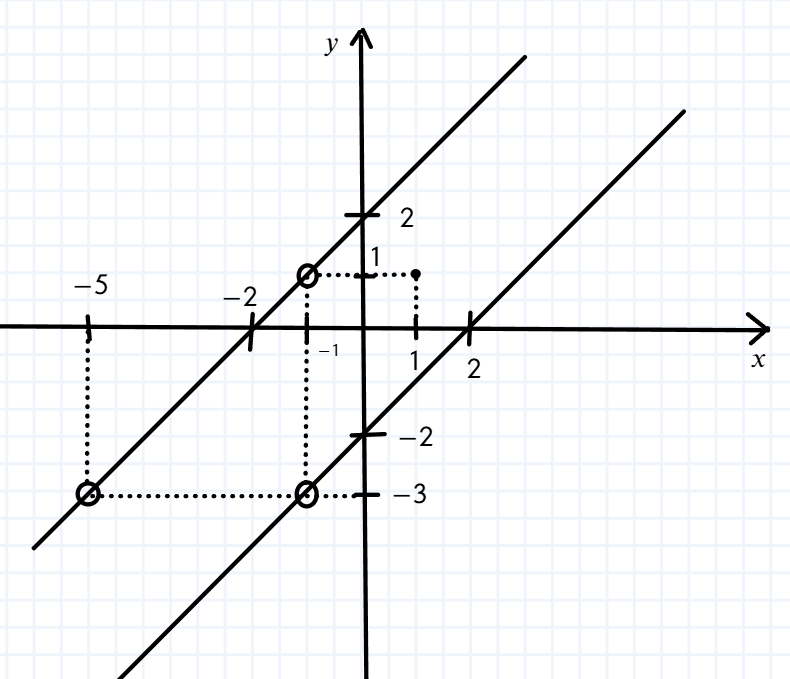
\includegraphics[scale=0.35]{gr7-97.png}}
\end{figure}\\
